%!TEX program = xelatex
\documentclass[a4paper, UTF8]{ctexrep}
\usepackage{ctex}
\usepackage{amsmath}
\usepackage{multirow}
\usepackage{amssymb}
\usepackage{graphicx}
\usepackage{geometry}
\usepackage{bm}
\usepackage{subfigure}
\usepackage{float}
\usepackage{array}
\usepackage{makecell}

\renewcommand\thesection{\arabic{section}}

\begin{document}
	\begin{titlepage}
		\centering
		\vspace{6cm}
		\LARGE{\textbf{Computer Vision HW1}}\\
		\vspace{4cm}
		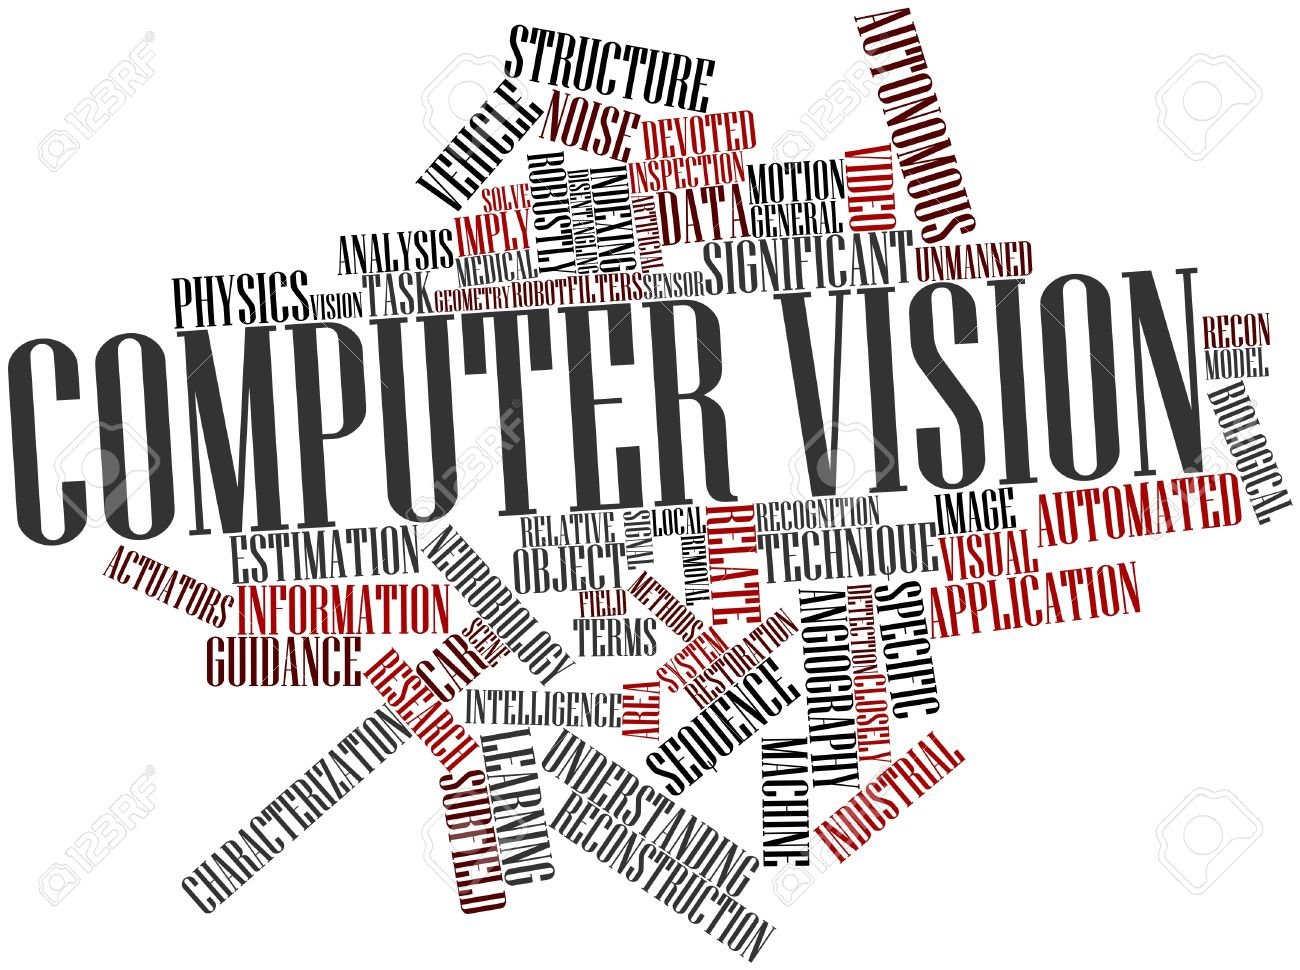
\includegraphics[width=0.8\textwidth]{cv.jpg}\\
		\vspace{5cm}
		\normalsize{安捷 1601210097}\\
		\normalsize{\today}
	\end{titlepage}
  \section{算法实现介绍}
  	在这一次作业中,我按照作业要求,分别实现了针对线性模型的RANSAC算法和针对线性最小二乘问题的RANSAC算法;我使用vl-feat工具包与我自己实现的RANSAC算法编写了图像拼接的函数和程序,并实现了任意多张图像的拼接;在作业中我还尝试了使用新老照片共同进行图像拼接的实验,没有取得比较好的效果。\\
  	在这里有几点算法实现的细节需要说明:
  	\begin{enumerate}
  		\item 为了使得图像最终的拼接效果反差不至于太大,起到一定的融合效果,我在算法中使用了两个操作,首先,对输入图像进行灰度均值的平均化,其次,对拼接的图像进行中值滤波以去除接缝处的灰度差异,考虑到最终对拼接图像的观察效果,我注释掉了中值滤波的代码;
  		\item 除了最终显示拼接结果的代码外,其余显示图像中间状态及匹配效果的图像显示代码我都进行了注释,这是因为cat操作在多图拼接的过程中会遇到图像大小不一致的异常,两幅图像拼接过程中,可以自行取消注释,即可看到拼接的中间过程;
  		\item 只需按照three\_image\_mosaic.m中的样式即可实现任意多张图像的拼接,但是当图像拼接达到一定规模之后,RANSAC算法的参数将难以适应,我尝试了拼接四张图像,在最后一张图像的拼接过程中始终没有得到比较好的结果,三张图像的拼接较为稳定;
  	\end{enumerate}
  \section{脚本参数设置}
	\begin{table}[htbp!]
	\centering
	\begin{tabular}{ccc}
	\hline
	参数名称 & 参数值 & 参数含义 \\
	\hline
	N & 4 & 求解线性最小二乘所需的最小点数 \\
	K & 300 & RANSAC算法迭代次数 \\
	T & 2 & 判断样本适合模型的误差阈值 \\
	D & 60 & 判断模型是否合适的样本数阈值 \\
	PEAK\_THRESH & 0.5 & SIFT算法阈值 \\
	EDGE\_THRESH & 10 & SIFT算法阈值 \\
	\hline
	\end{tabular}
	\caption{two\_image\_mosaic.m参数表}
	\end{table}

	\section{运行结果}
	\clearpage
		\begin{figure}[htbp!]
			\centering
			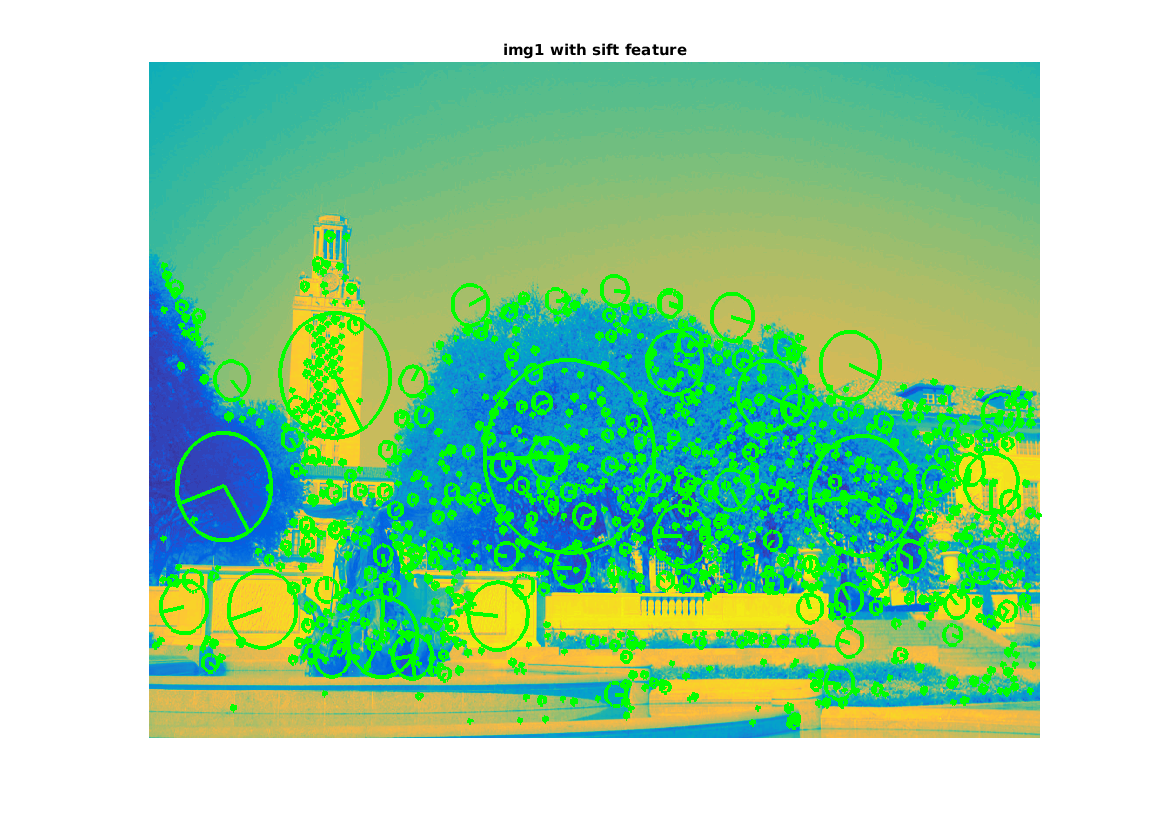
\includegraphics[width = \textwidth]{hw2_fig1.png}
			\caption{左图像SIFT检测子结果}
			\label{fig:figure1}
		\end{figure}
		\clearpage
		\begin{figure}[htbp!]
			\centering
			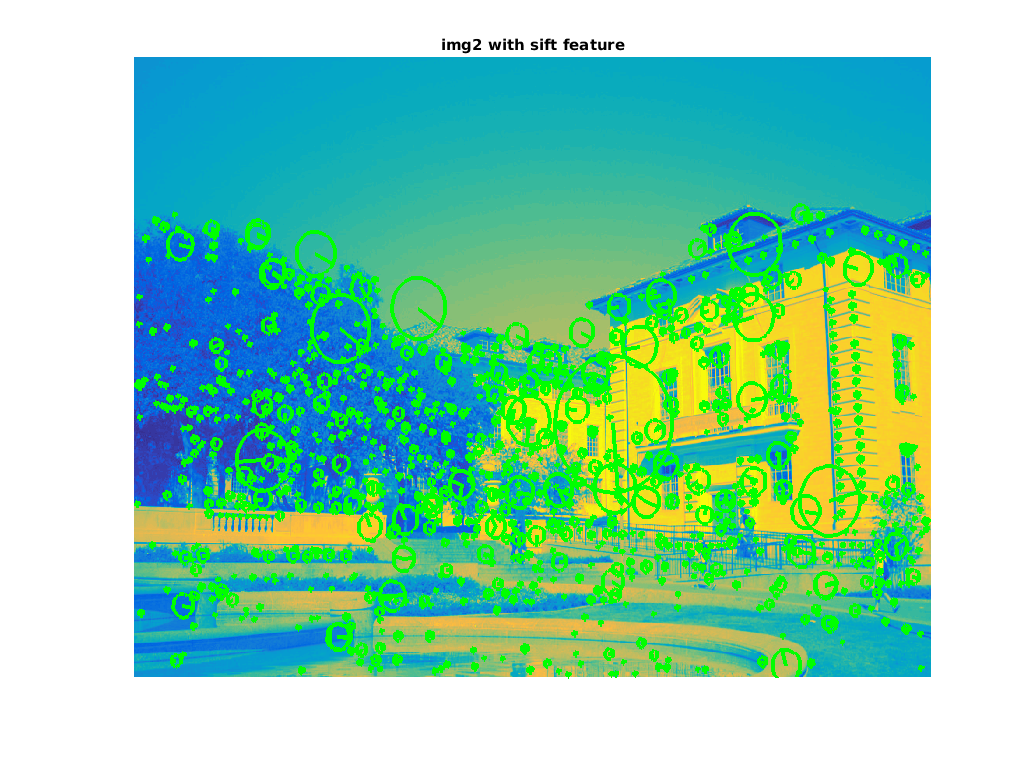
\includegraphics[width = \textwidth]{hw2_fig2.png}
			\caption{右图像SIFT检测子结果}
			\label{fig:figure1}
		\end{figure}
		\clearpage
		\begin{figure}[htbp!]
			\centering
			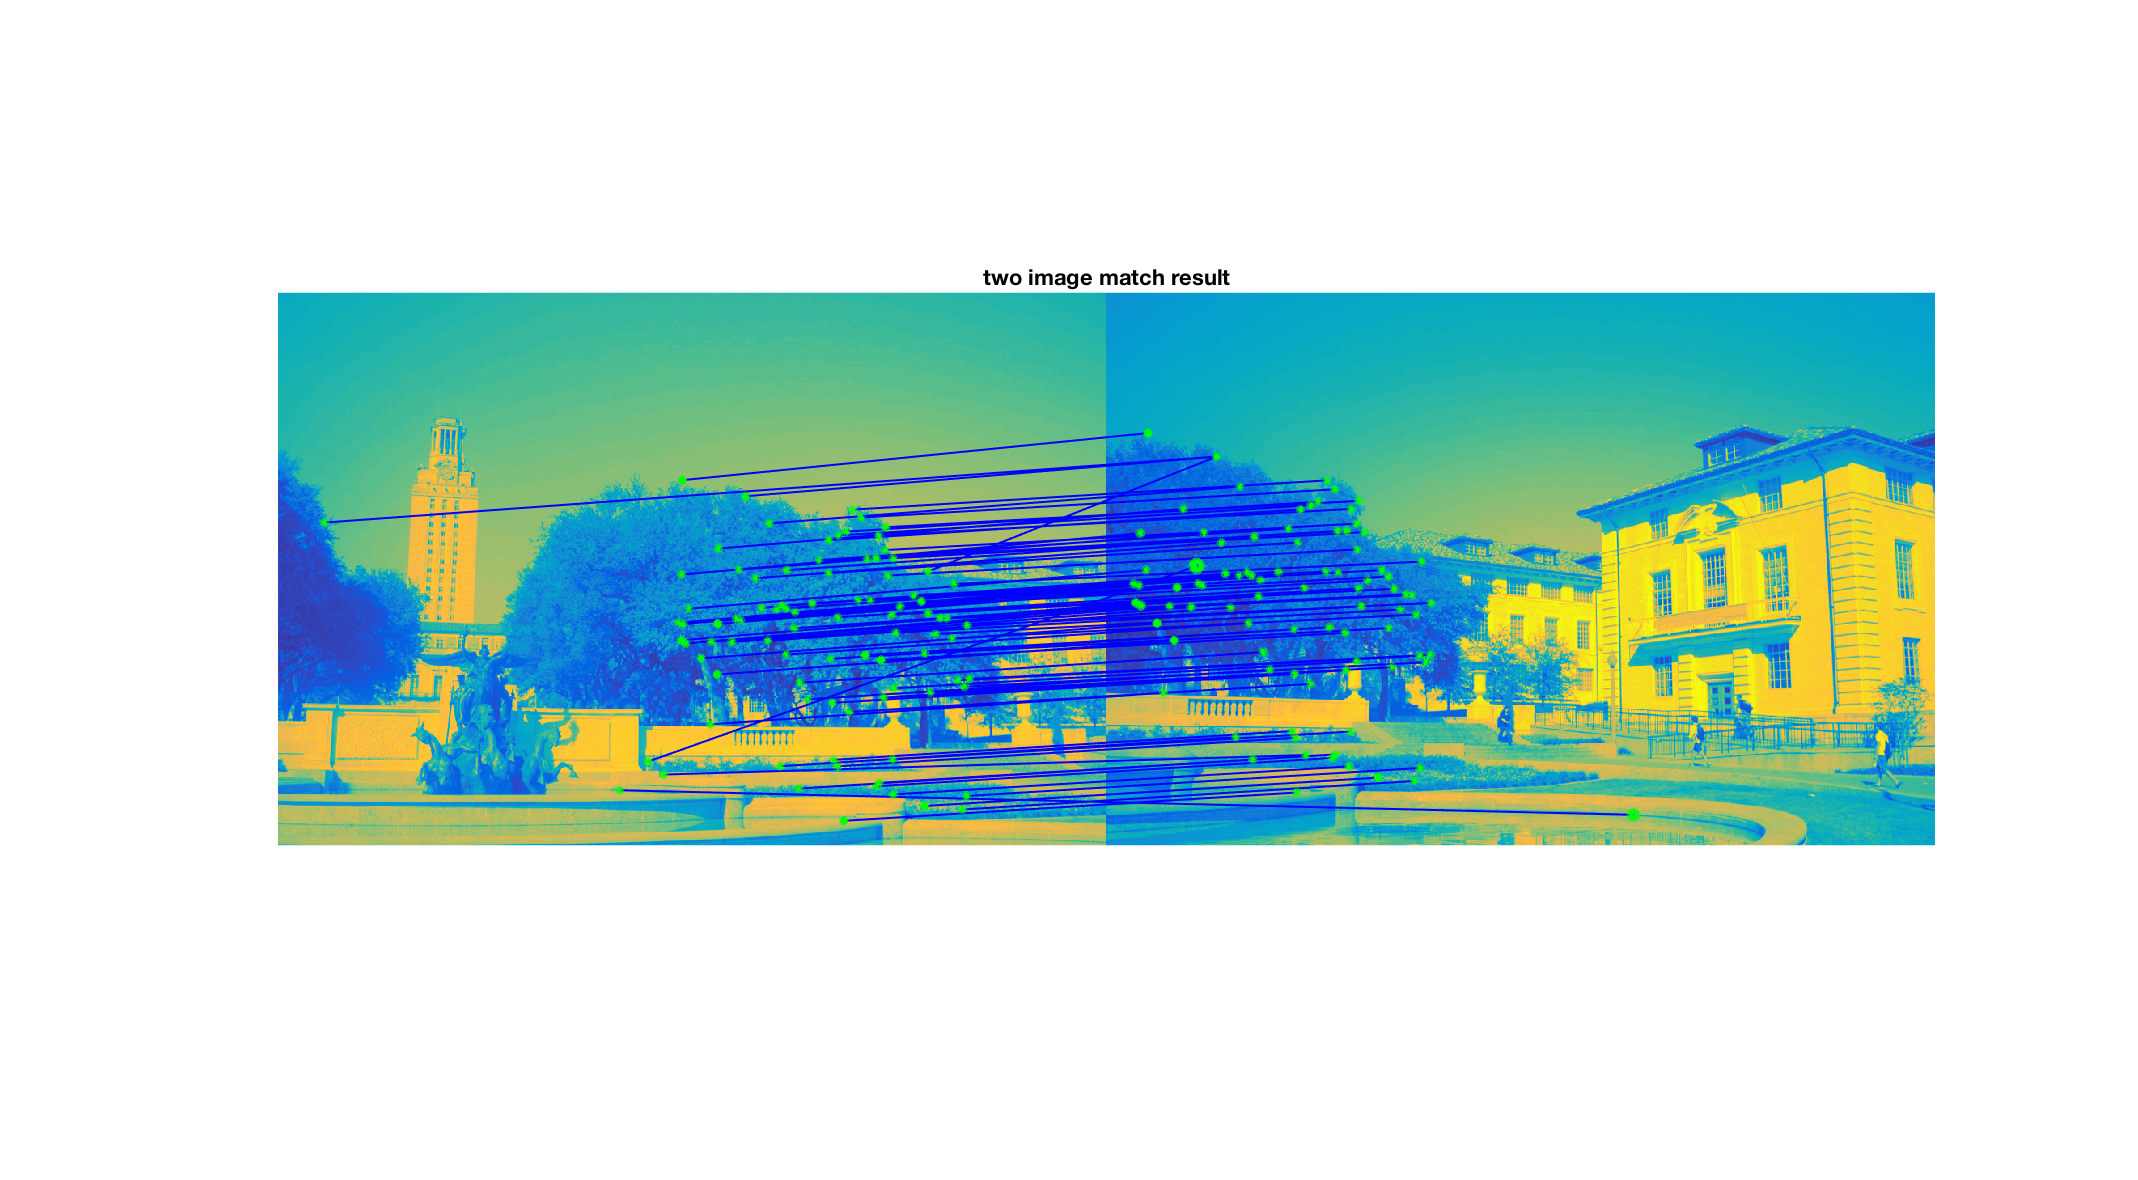
\includegraphics[width = \textwidth]{hw2_fig3.png}
			\caption{SIFT匹配结果}
			\label{fig:figure1}
		\end{figure}
		\clearpage
		\begin{figure}[htbp!]
			\centering
			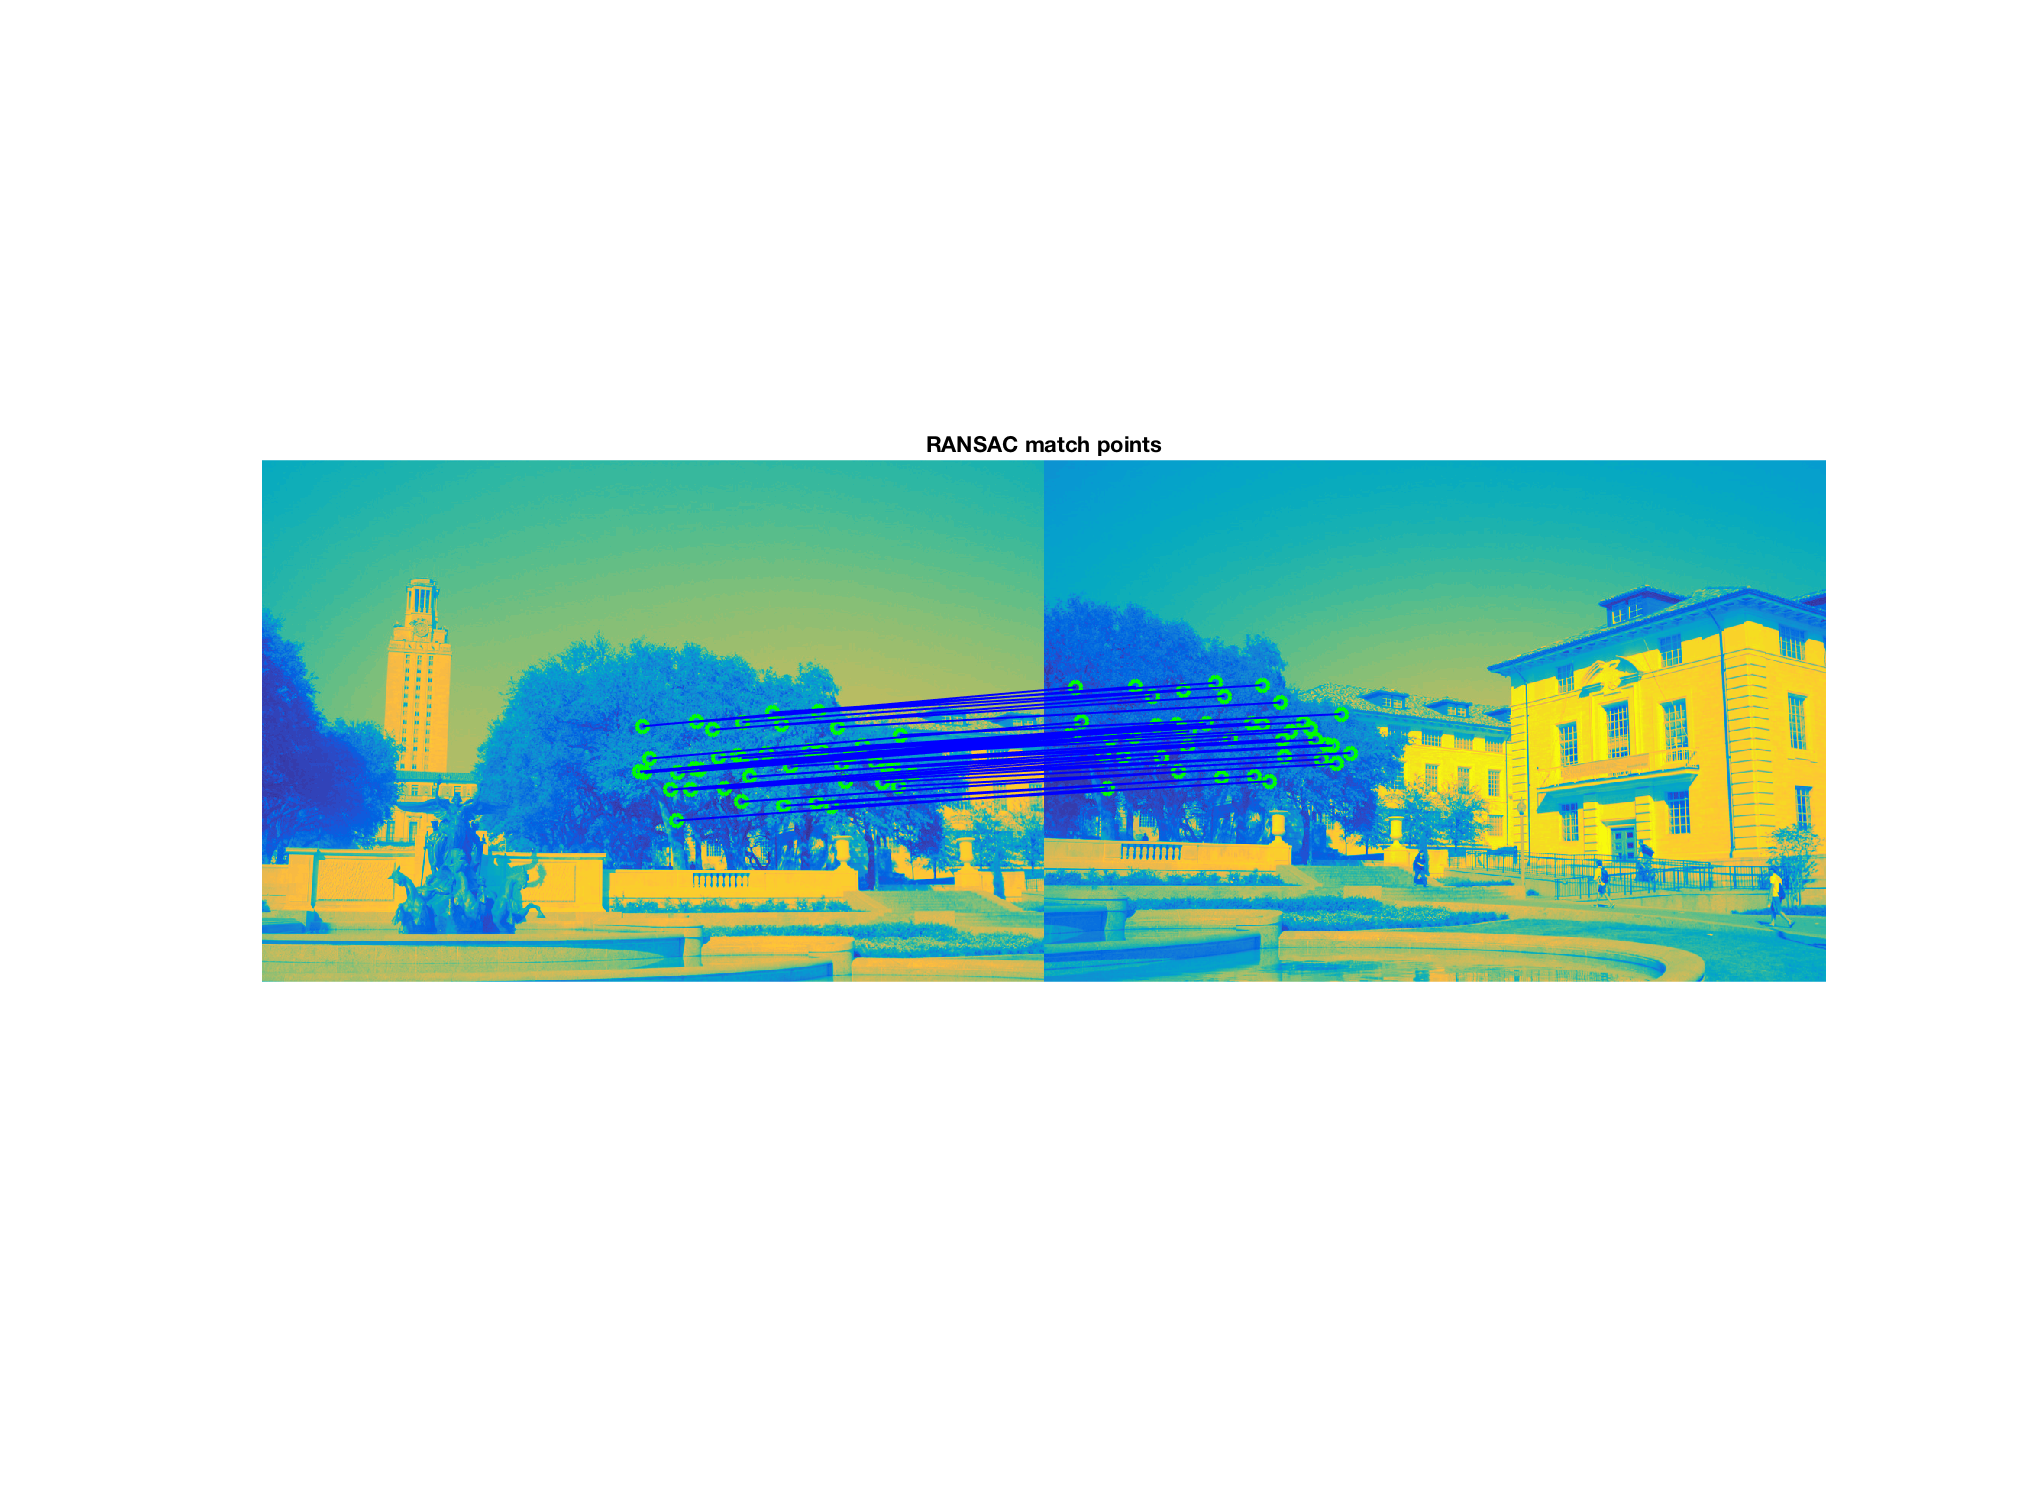
\includegraphics[width = \textwidth]{hw2_fig4.png}
			\caption{RANSAC匹配结果}
			\label{fig:figure1}
		\end{figure}
		\clearpage
		\begin{figure}[htbp!]
			\centering
			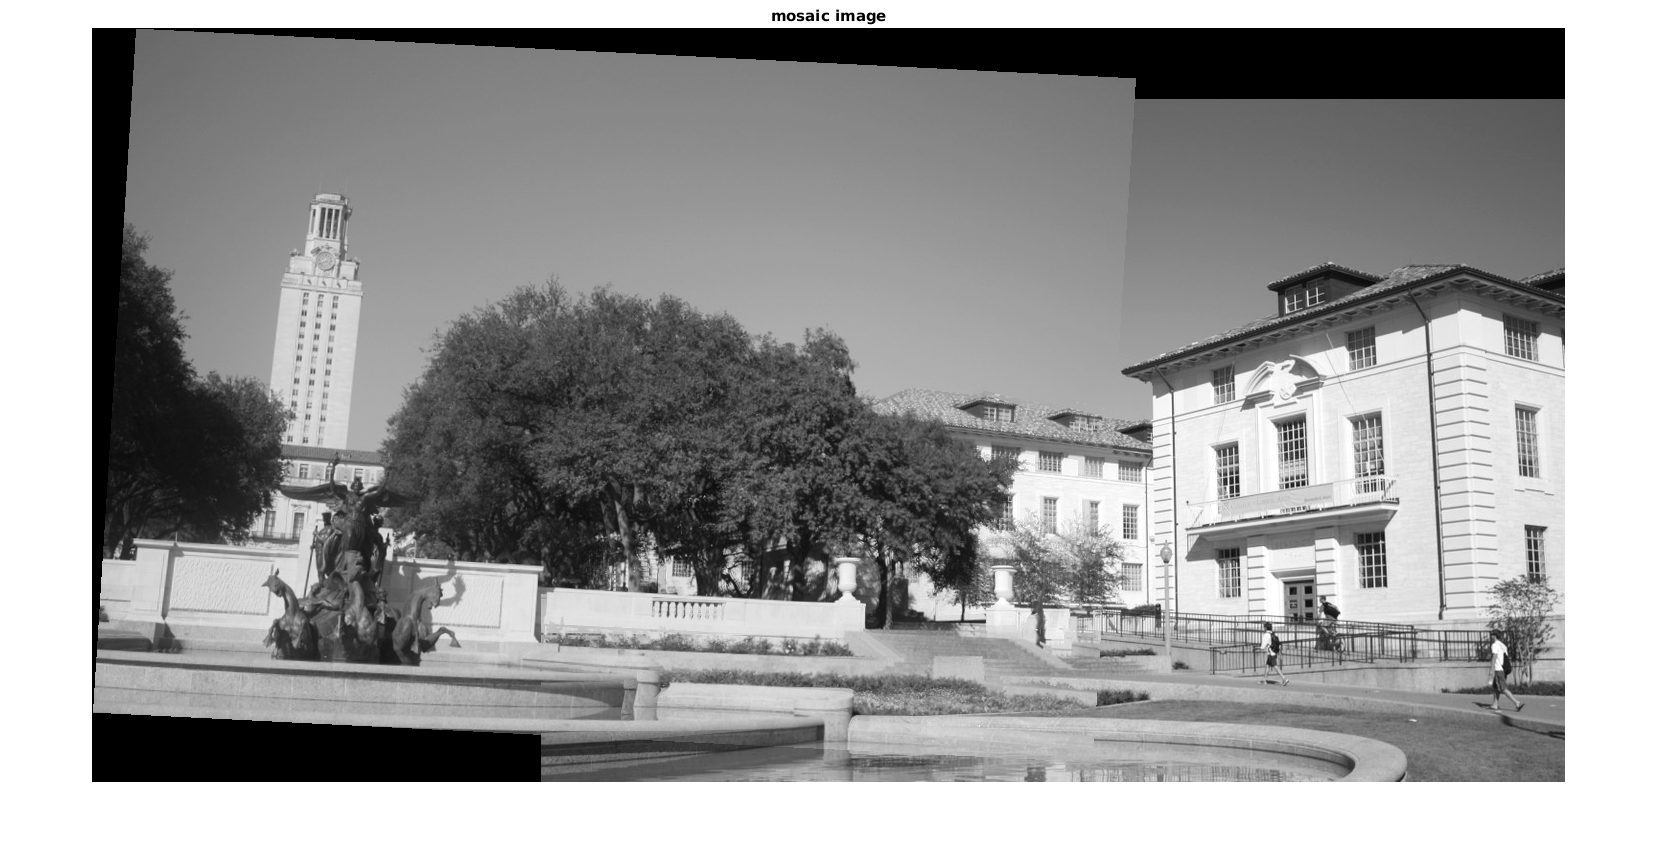
\includegraphics[width = \textwidth]{hw2_fig5.png}
			\caption{两图像拼接结果}
			\label{fig:figure1}
		\end{figure}
		\begin{figure}[htbp!]
			\centering
			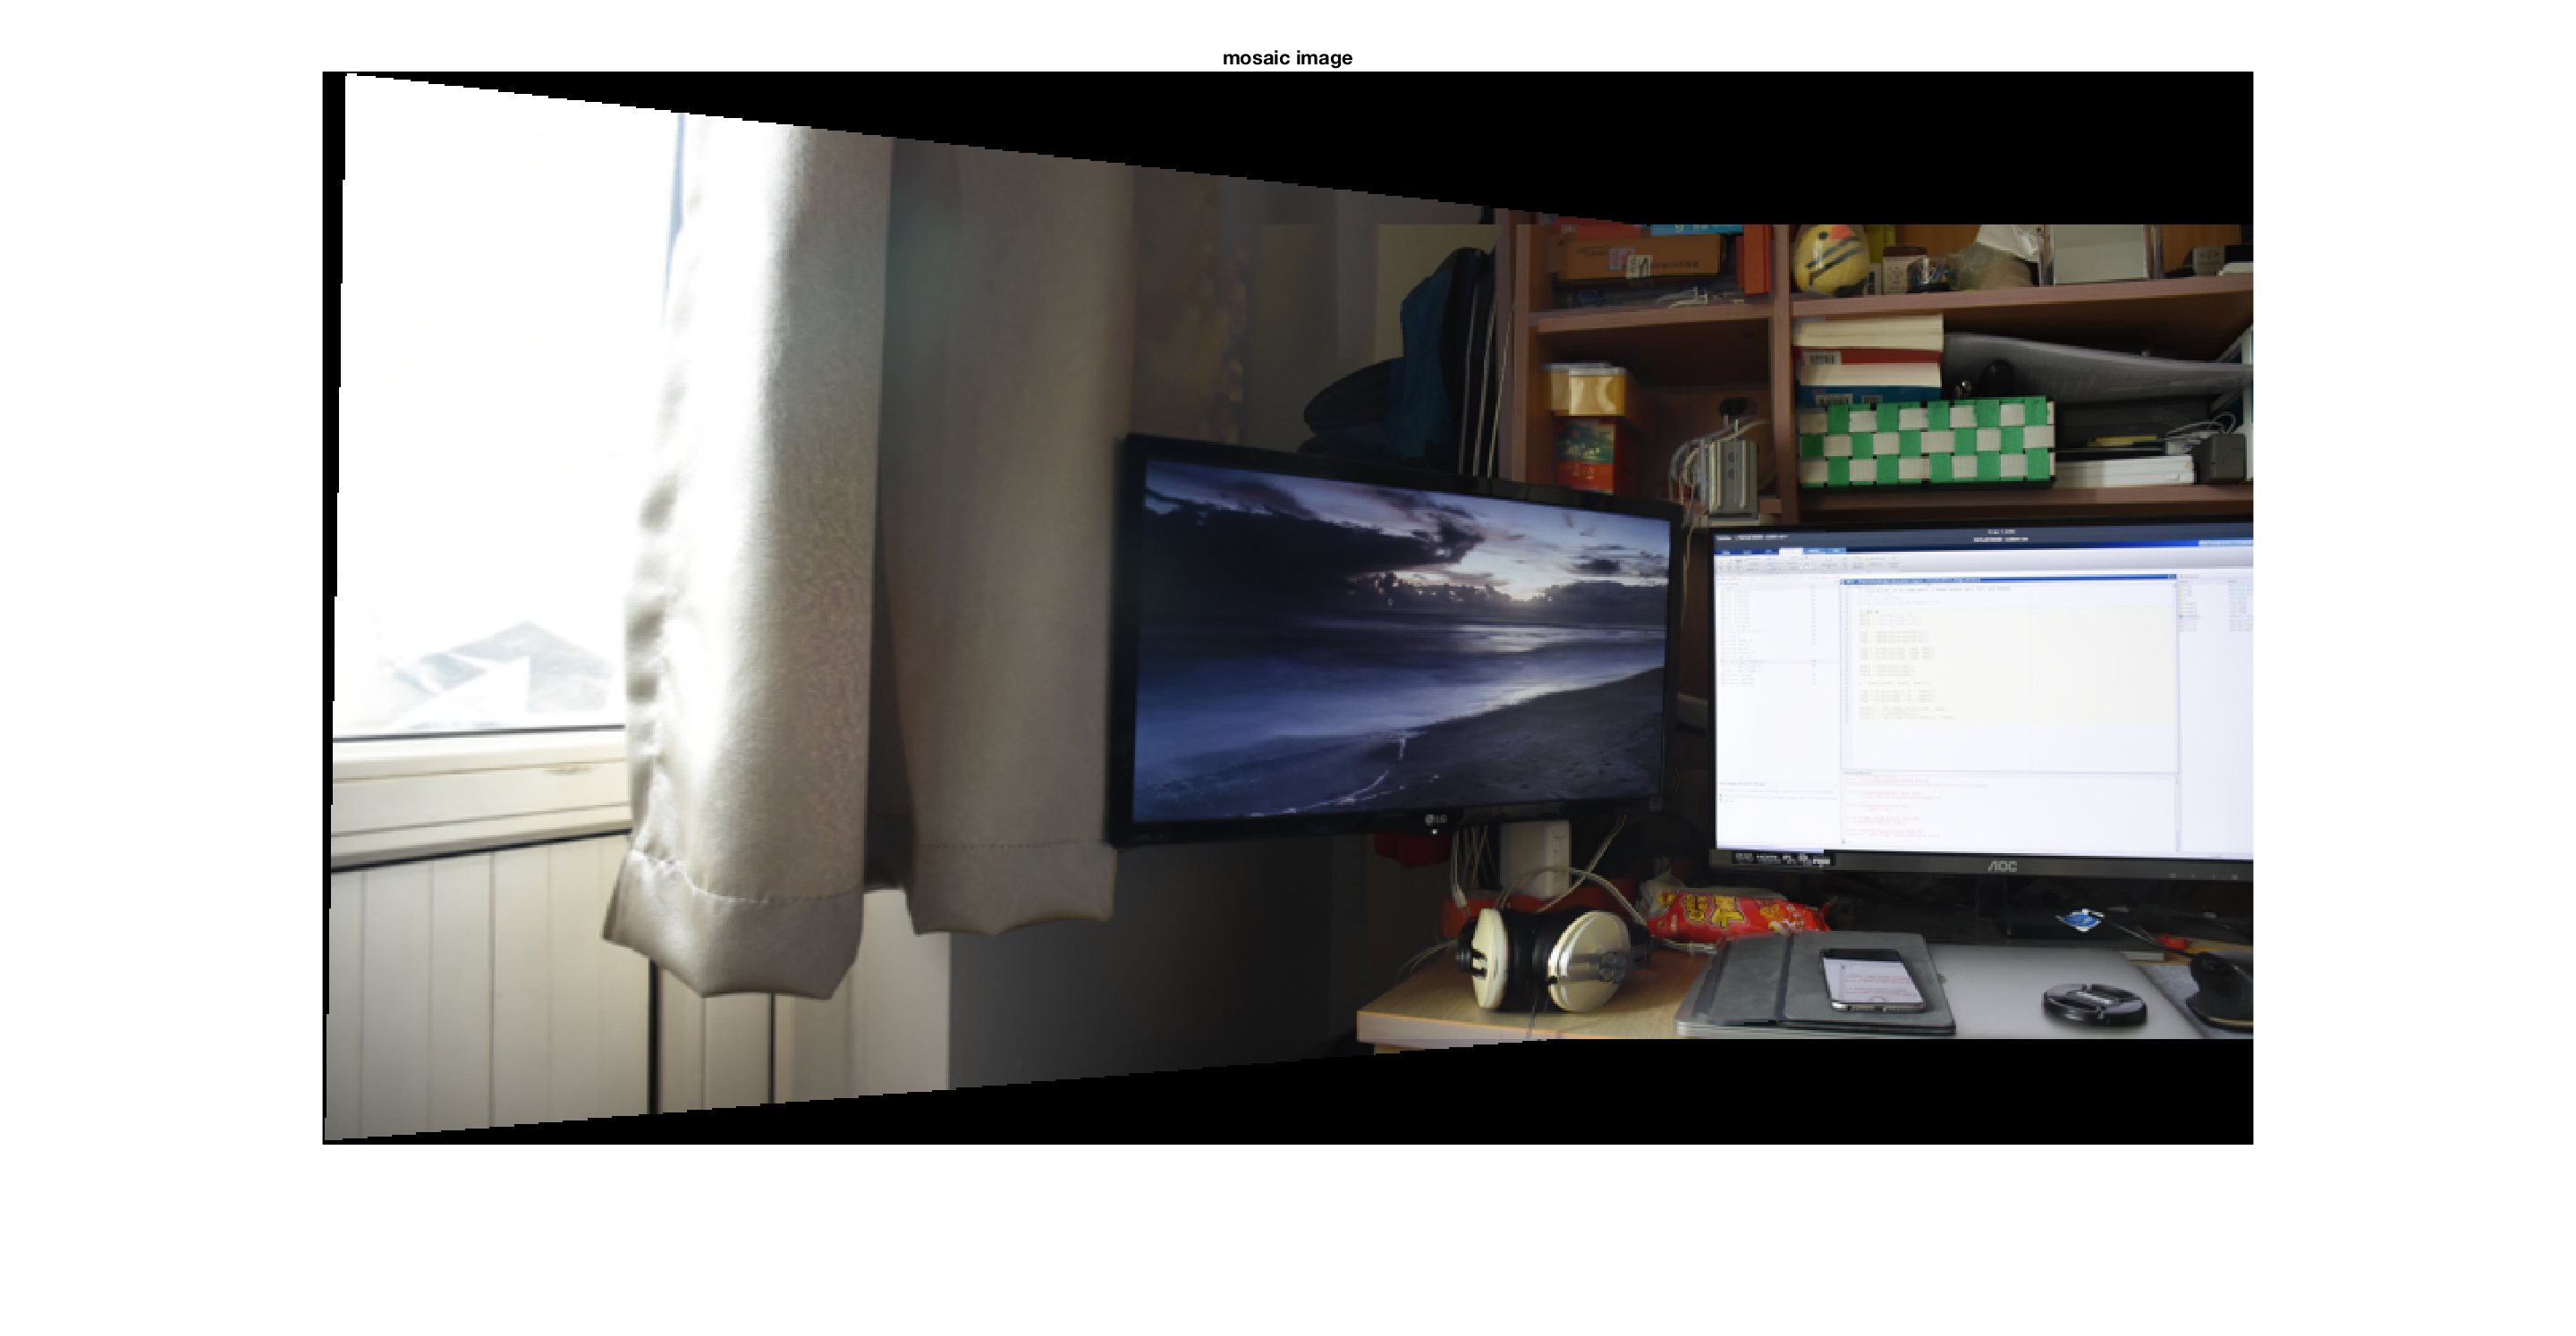
\includegraphics[width = \textwidth]{hw2_fig6.png}
			\caption{三图像拼接结果1}
			\label{fig:figure1}
		\end{figure}
		\clearpage
		\begin{figure}[htbp!]
			\centering
			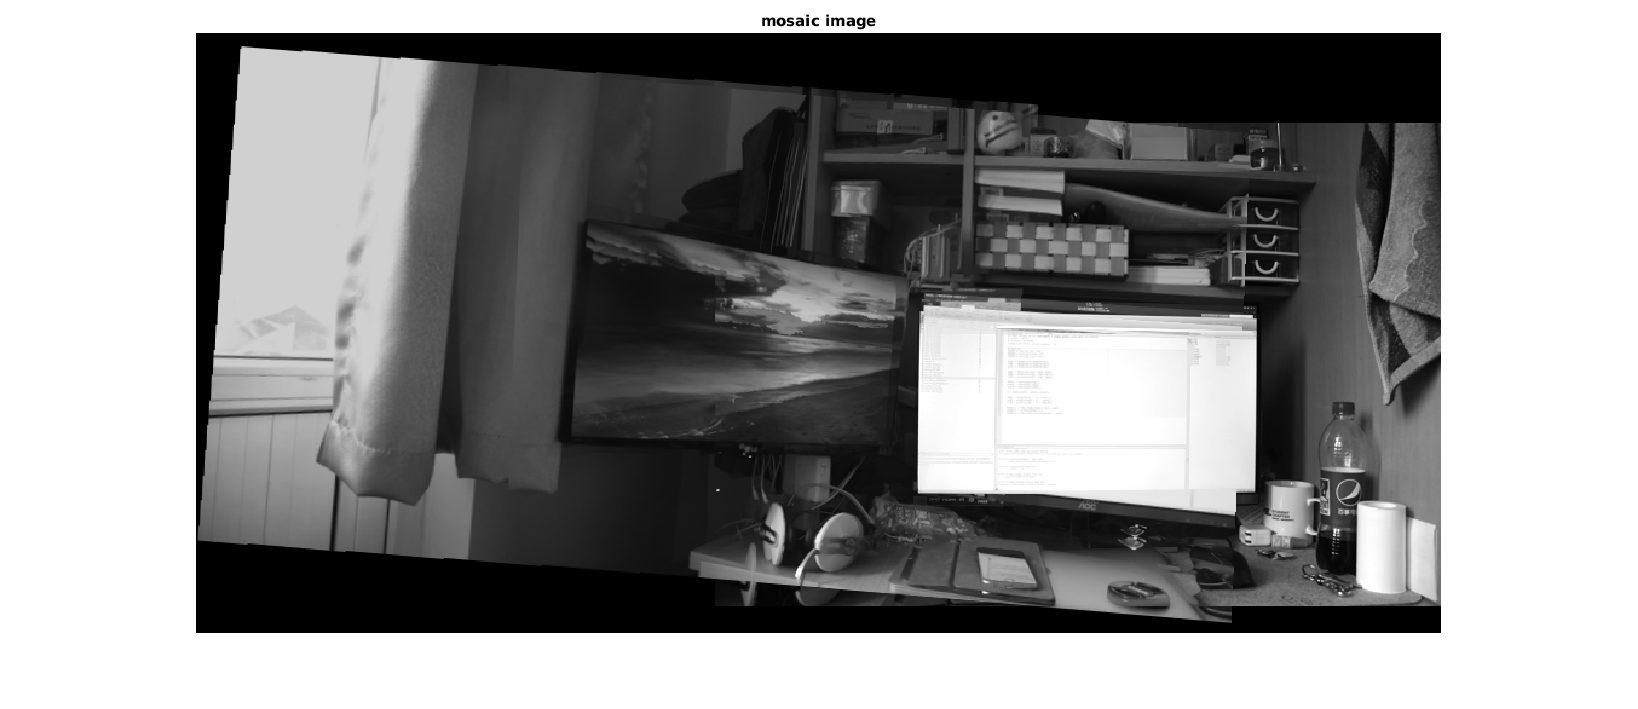
\includegraphics[width = \textwidth]{hw2_fig7.png}
			\caption{三图像拼接结果2}
			\label{fig:figure1}
		\end{figure}
		
	\section{结论}
	\begin{enumerate}
		\item SIFT算子与RANSAC算法结合可以实现较为精确的图像拼接;
		\item RANSAC算法对于参数非常敏感,尤其是误差阈值T和模型最小支持样本阈值D,我在实现的过程中尝试了多次调整参数才在三张图像的拼接中得到一个可以接受的结果,我观察到,对于两张图像的拼接,参数的敏感性稍微可以减弱;
		\item 上述算法能够更好的工作且具有较高的鲁棒性,但是对于图像的尺度差别过大的情形下,由于SIFT算子不再可以很好的表示两者尺度差异巨大的特征,算法不work,这部分的数值实验可以参看two\_image\_mosaic\_test.m中新旧图像拼接的部分;
	\end{enumerate}

  \section{软件版本及测试平台信息}
    这部分内容请参看源代码所在文件夹内的REAME文件。
\end{document}